Now that I have established some facts about motor proteins as well as specifics about dynein's many odd behaviors, we may begin our discussion of how to construct and test a physical model for its motion. First, we note that dynein's large mass of roughly 2MDa \cite{johnson_structure_1983} as compared to similar motor proteins such as Kinesin (a few hundred kDa) \cite{liao_kinesin_1998} exaggerates the effect of interactions with the  aqueous environment of the cell. This results in a much more significant drag force as well as a random element from water molecule collisions that changes the overall dynamics of the system. The set of equations governing this motion is called Brownian dynamics and is what we use to simulate the trajectory of dynein along the microtubule. 
	\section{Brownian dynamics}
	To model dynein we treat its various domains (binding, motor, and tail) as spheres held together by massless rigid-rods. In general, the dynamics of a constant mass particle are governed by Newton's second law
	\begin{equation}
		\sum_i \mathbf{F}_i = \dot{\mathbf{p}} = m\ddot{\mathbf{x}}
	\end{equation}
	Thus, determining the dynamics of a system boils down to describing the various forces which act upon it and then solving the resulting differential equation for some set of initial conditions. For small particles in a solvent, there are three important forces to consider. The first is linear drag, which we write as 
	\begin{equation}
		F_\text{drag} = -\gamma\dot{\mathbf{x}}
	\end{equation}
	so that the drag force is proportional to the velocity by a factor $\gamma$. For a spherical particle of radius $a$ moving through a solvent with liquid viscosity $\eta$ this was derived by Stoke to be 
	\begin{equation}
		\gamma = 6\pi\eta a
	\end{equation}
	
	
	The second characteristic force of Brownian dynamics is a random force due to density fluctuations in the solvent which we denote $F_\text{rand}$. Finally, we might also consider how individual particles interact with each other through some interaction force. For us, this will be accomplished through the rigid rods that outline the structure of the protein by fixing the inter-domain distances via tension. Putting all of these forces together results in what is often called the \textit{Langevin Equation}.
	\begin{equation}
		 -\gamma\dot{\mathbf{x}}+\mathbf{F}_\text{rand} + \mathbf{F}_\text{interact} = m\ddot{\mathbf{x}} 
	\end{equation}
	
	If we assume further that $|\gamma\dot{\mathbf{x}}|\gg |m\ddot{\mathbf{x}}|$, or in other words, we take the limit of strong drag, then we arrive at the definition of Brownian Dynamics. This allows us to neglect the acceleration term resulting in the following differential equation
	\begin{equation}
		\dot{\mathbf{x}} = \frac{1}{\gamma}\left( \mathbf{F}_\text{interact} + \mathbf{F}_\text{rand} \right)
	\end{equation}
	which we must now solve for the equations of motion of our model. 
	
	
	\section{A Simplified Model for Dynein}
	As mentioned, we model dynein as a system of spherical domains held together by massless rigid-rods with the whole system moving according to Brownian dynamics. The random forces on each domain are responsible for diffusing the system and creating the expected chaotic motion, but in order to have dynein prefer walking towards one side of the microtubule, as is the case for real dynein, we need to impose some \textit{extra} structure on the protein. 
	
	\begin{figure}[hbt!]
		\centering
		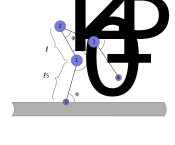
\includegraphics[angle=-90, width=0.6\columnwidth]{torque_angles}
		\caption{Example of dynein in the one bound configuration with torque angles $\{\varphi_i\}$ shown.}
		\label{fig:torque angles}
	\end{figure}
	
	To do this we steer each domain towards an equilibrium configuration by a Hooke's law restorative torque with magnitude of the following form
	\begin{equation}
		\Gamma_i = -c_i\left(\varphi_i-\varphi_{i,\text{eq}}\right)
	\end{equation}
	Here the $c_i$ are spring constants (a free parameter of the model) and the set $\{\varphi_i\}$ are the angles measured between the $i-1$ and $i+1$ domains. Equally useful is the harmonic energy associated with each torque. These are given by
	\begin{equation}
		U_i = \frac{1}{2}c_i(\varphi_i-\varphi_{i,\text{eq}})^2
	\end{equation} 
	
	Real dynein is composed of a pair of identical heavy chains. Therefore, our angle convention is chosen starting at the $0^{th}$ domain in figure \ref{fig:torque angles}. The same convention is then repeated for the second leg with the following correspondence 
	\begin{align}
		\varphi_{0,eq} &\longleftrightarrow \varphi_{4,eq} \\ 
		\varphi_{1,eq} &\longleftrightarrow \varphi_{3,eq}
	\end{align}
	where the angles $\{\varphi_{i, \text{eq}}\}$ are the preferred angles of the system as illustrated in figure \ref{fig:torque angles}. The torques on each domain are related to forces by 
	\begin{equation}
		\mathbf{\Gamma} = \mathbf{r}\times\mathbf{F}
	\end{equation}
	so that knowing the distance between each domains means that we have specified each of the $\mathbf{\Gamma}_i$ and $\mathbf{r}_i$. In order to dynamically move each domain we must invert equation 4.10 to determine $\mathbf{F}_i$, however there is no unique way to invert such a cross product. Therefore, we must specify an algorithm for determining the forces that result from each torque. 
	
	\section{Calculating Forces and Torques}
	Here I will discuss in detail how we calculate the forces and show how this is done in code
	
	
	
	\section{Equations of Motion}
	Now that we have specified the forces, the dynamics of each domain are determined by equation 4.5 so that in order to simulate the complicated structure we must solve a system of coupled first order differential equations. In doing so, it is convenient to introduce two states to distinguish between dynein's stepping and when both of its binding domains are attached to the microtubule. We shall refer to these configurations hereafter as the one bound state and the both bound state. 
	
	In the one bound state, all but one of the domains are free to diffuse while the last is attached to the microtubule. In the both bound state, both binding domains are attached. This slight difference in geometry between the two scenarios leads to two sets of equations for motion that differ slightly. The following section details the derivation of these equations of motion. 
	
		\subsection{The one bound state}
		Figure \ref{fig:one bound} illustrates dynein in the one bound state with new angles $\{\theta_i\}$ chosen for convenience of calculation and computation.\\
		\begin{figure}[!hbt]
			\centering
			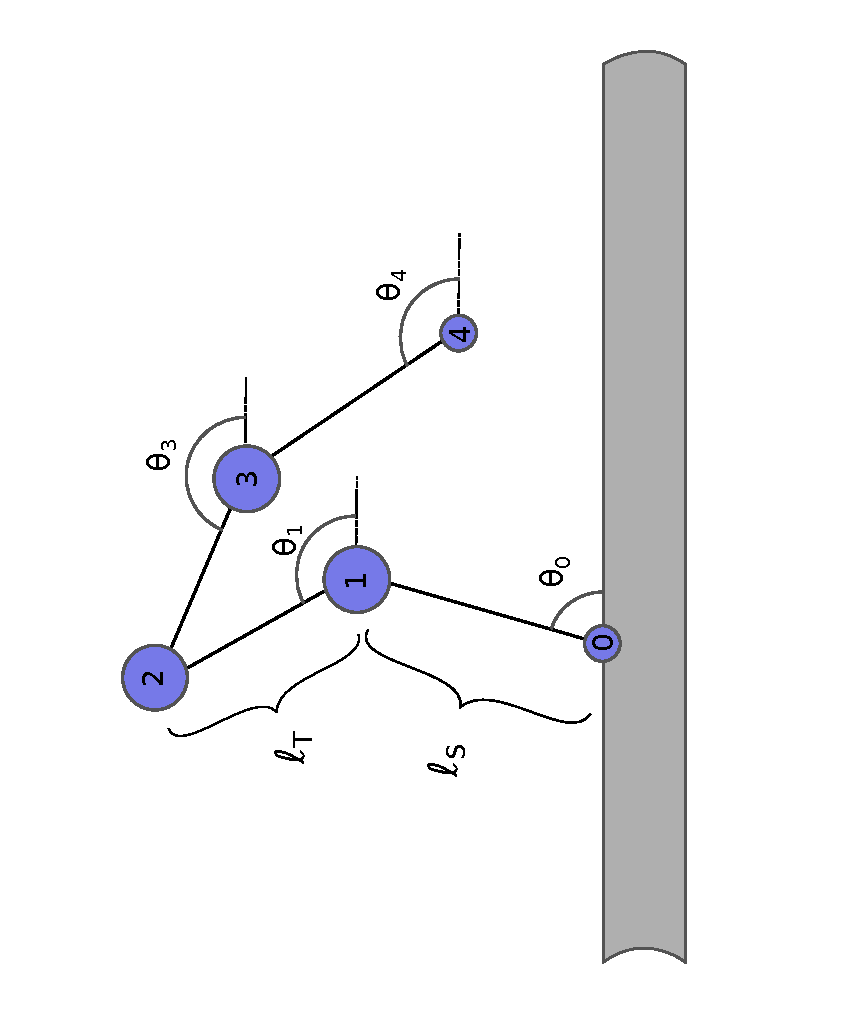
\includegraphics[angle=-90,width=0.75\columnwidth]{onebound}
			\caption{The dynein model in the one bound state }
			\label{fig:one bound}  
		\end{figure}
		
		\noindent Here $\ell_S, \ell_T$ are fixed stalk and tail lengths. With some simple trigonometry, the positions of each domain are given by
		\begin{align}
		x's \quad &\begin{cases}
		x_0 = x_\text{bound} \\
		x_1 = x_0 + \ell_S \cos\theta_0 \\
		x_2 = x_1 + \ell_T \cos\theta_1 \\
		x_3 = x_2 + \ell_T \cos(\pi-\theta_3) = x_2 - \ell_T\cos\theta_3 \\
		x_4 = x_3 + \ell_S \cos(\pi-\theta_4) = x_3 - \ell_S\cos\theta_4
		\end{cases} &
		y's \quad &\begin{cases}
		y_0 = 0 \\
		y_1 = y_0 + \ell_S\sin\theta_0 \\
		y_2 = y_1 + \ell_T\sin\theta_1 \\
		y_3 = y_2 - \ell_T\sin\theta_3 \\
		y_4 = y_3 - \ell_S\sin\theta_4 
		\end{cases}
		\end{align} 
		
		\noindent Because equation (3.5) relates the forces on each domain to its velocity we need the time derivative of the above equations. 
		\begin{align}
		\dot{x}'s \quad \begin{cases}
		\dot{x}_0 = 0 \\
		\dot{x}_1 = \dot{x}_0-\ell_S\sin\theta_0 \dot{\theta}_0 \\
		\dot{x}_2 = \dot{x}_1-\ell_T\sin\theta_1 \dot{\theta}_1 \\
		\dot{x}_3 = \dot{x}_2+\ell_T\sin\theta_3 \dot{\theta}_3 \\
		\dot{x}_4 = \dot{x}_3+\ell_S\sin\theta_4 \dot{\theta}_4
		\end{cases} &
		\dot{y}'s \quad \begin{cases}
		\dot{y}_0 = 0 \\
		\dot{y}_1 = \dot{y}_0 + \ell_S\cos\theta_0\dot{\theta}_0 \\
		\dot{y}_2 = \dot{y}_1 + \ell_T\cos\theta_1\dot{\theta}_1 \\
		\dot{y}_3 = \dot{y}_2 - \ell_T\cos\theta_3\dot{\theta}_3 \\
		\dot{y}_4 = \dot{y}_3 - \ell_S\cos\theta_4\dot{\theta}_4
		\end{cases} 
		\end{align}
		
		The Brownian motion equation (3.5) also defines the velocity on domain. 
		
		 
		\subsection{The both bound state}
		 
		\section{Determining constants of the model}
		The stalk and tail lengths $\ell_S, \ell_T$ as well as a set of equilibrium angles $\{\varphi_{i,\text{eq}}\}$ were determined by examining microscopy images of dynein in various configurations. 
		\begin{figure}[hbt!]
			\centering
			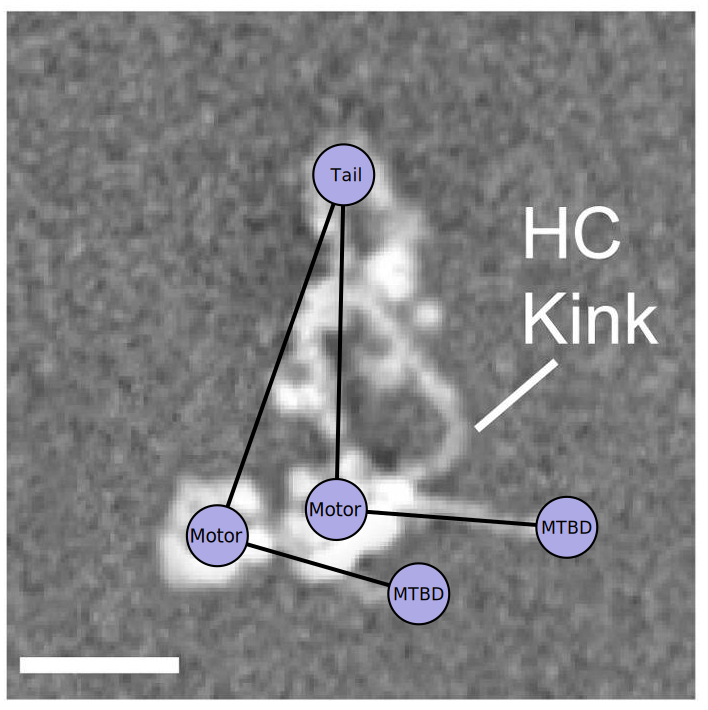
\includegraphics[width=0.3\columnwidth]{schematic-2-superimposed}
			\caption{Our model superimposed over microscopy image of Dynein \textbf{NOTE: add source} for determining lengths and equilibrium angles} 
			\label{fig:superimpmosed}
		\end{figure}
	\section{The Code}
		\subsection{The Random Force}
